\documentclass[12pt,aspectratio=169]{beamer}

\usetheme[
    sectionpage=progressbar,
    subsectionpage=progressbar,
    progressbar=frametitle
]{metropolis}

\definecolor{blue-grey-900}{HTML}{263238}
\definecolor{deep-orange-500}{HTML}{FF5722}
\setbeamercolor{normal text} {fg=blue-grey-900,   bg=white}
\setbeamercolor{alerted text}{fg=deep-orange-500}

\usepackage{graphicx}
\usepackage{hyphenat}
\usepackage[normalem]{ulem}

\usepackage{polyglossia}
\setdefaultlanguage[variant=british]{english}
\usepackage[english=british]{csquotes}

\usepackage{fontspec}
\setmainfont{Lucida Sans OT}
\setsansfont[Scale=MatchLowercase]{Lucida Sans OT}
\setmonofont[Scale=MatchLowercase]{Lucida Console DK}
\defaultfontfeatures{Ligatures=TeX}

\title{Lessons learned from teaching Data Science}
\author{Gianluca Campanella}
\date{21\textsuperscript{st} April 2018}

\begin{document}

\maketitle

\begin{frame}{Hello!}
    \begin{center}
        \LARGE%
        My name is \textbf{Gianluca}
        {\fontspec{Gentium}\textcolor{gray}{[dʒanˈluːka]}}
    \end{center}
\end{frame}

\begin{frame}{What I do nowadays}
    \LARGE%
    \only<1>{%
        \begin{center}
            I'm a Data Scientist at \\[\bigskipamount]
            
\includegraphics[height=2.5em]{figures/microsoft} \\[\medskipamount]
            in \textbf{Algorithms and Data Science}
        \end{center}}
    \only<2>{%
        \begin{center}
            I also run my own company \\[\bigskipamount]
            
\includegraphics[height=2.5em]{figures/estimand} \\[\medskipamount]
            that provides \\
            \textbf{Data Science training and mentoring}
        \end{center}}
\end{frame}

\begin{frame}{How I got into teaching}
    \LARGE%
    \begin{center}
        It all started at \\[\bigskipamount]
        
\includegraphics[height=2.5em]{figures/icl}
    \end{center}
\end{frame}

\begin{frame}{Today I want to talk to you about\ldots}
    \LARGE%
    \begin{enumerate}
        \setlength{\itemsep}{\bigskipamount}
        \item The skills gap in Data Science
        \item The Data Science potential
        \item How we implement all this
    \end{enumerate}
\end{frame}

\begin{frame}{What I mean by `Data Science'}
    \only<1>{%
        \begin{center}
            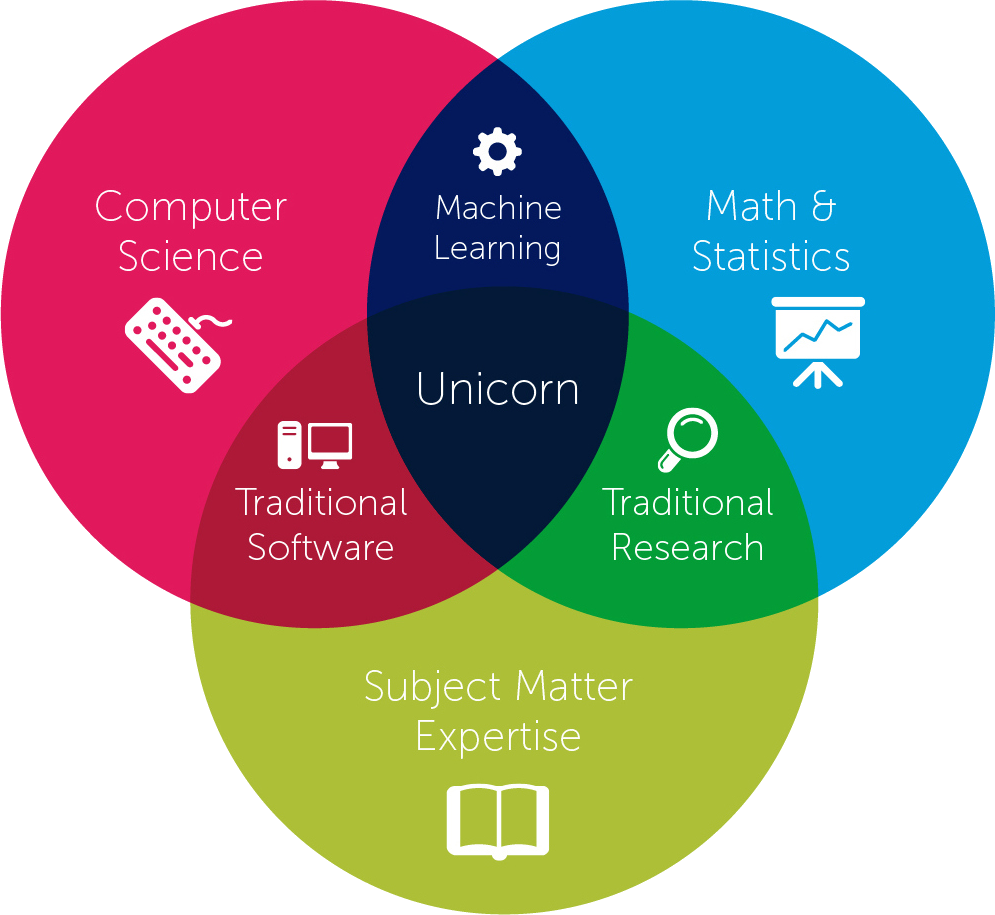
\includegraphics[height=0.8\textheight]{figures/data_science_venn_diagram} \\
            {\scriptsize%
             From S.\ Geringer (originally from D.\ Conway)}
        \end{center}}
    \only<2>{%
        \begin{center}
            \Large\bf%
            Data\hyp{}driven decision\hyp{}making
        \end{center}
        \vfill
        \begin{itemize}
            \setlength{\itemsep}{\medskipamount}
            \item Focus is on the problem\hyp{}solving process
            \item Multidisciplinary but domain\hyp{}centric
            \item Tools are secondary
        \end{itemize}}
\end{frame}

\begin{frame}{The Data Science skills gap}
    \begin{center}
        \Large\it%
        The shortage of data scientists is becoming \\[\medskipamount]
        a serious constraint in some sectors.
    \end{center}
    \vfill
    \begin{flushright}
        --- T.\ H.\ Davenport and D.\ J.\ Patil \\
            \textit{Harvard Business Review} (2012)
    \end{flushright}
\end{frame}

\begin{frame}{How do we close the skills gap?}
    \only<1>{%
        \begin{columns}
            \begin{column}{0.5\textwidth}
                \centering%
                {\Large\bf%
                 Higher Ed} \\[\medskipamount]
                `Traditional' degrees \\[\bigskipamount]
                \begin{itemize}
                    \setlength{\itemsep}{\medskipamount}
                    \item Lots of theory
                    \item Take a while to catch up
                    \item More recognition?
                \end{itemize}
            \end{column}
            \begin{column}{0.5\textwidth}
                \centering%
                {\Large\bf%
                 Up\hyp{}skilling} \\[\medskipamount]
                Bootcamps, MOOCs\ldots \\[\bigskipamount]
                \begin{itemize}
                    \setlength{\itemsep}{\medskipamount}
                    \item Mostly hands\hyp{}on
                    \item Adapt faster
                    \item `Show your skills'
                \end{itemize}
            \end{column}
        \end{columns}}
    \only<2>{%
        \Large%
        How do we ensure\ldots
        \begin{itemize}
            \setlength{\itemsep}{\medskipamount}
            \item Relevance?
            \item Quality?
            \item Consistency?
        \end{itemize}}
\end{frame}

\begin{frame}{The \emph{actual} question}
    \LARGE%
    \only<1>{%
        \begin{center}
            How do we realise \\
            the potential of Data Science?
        \end{center}}
    \only<2>{%
        \begin{center}
            \textcolor{gray}{\sout{How do we realise}} \\
            What even is \\
            the potential of Data Science?
        \end{center}}
\end{frame}

%\section{Potential}

\begin{frame}{The Data Science potential}
    \Large%
    Data Science promises\ldots
    \begin{itemize}
        \setlength{\itemsep}{\medskipamount}
        \item Automation
        \item Risk minimisation
        \item Innovation
    \end{itemize}
\end{frame}

\begin{frame}{How do we realise this potential?}
    \only<1>{%
        \begin{center}
            \LARGE%
            Data Science needs to be \\[\bigskipamount]
            {\Huge\textbf{embedded}} \\[\bigskipamount]
            within companies and processes
        \end{center}}
    \only<2>{%
        \Large%
        This means\ldots
        \begin{itemize}
            \setlength{\itemsep}{\medskipamount}
            \item Build, don't buy
            \item Cultivate internally, don't outsource
            \item Humans in the loop
        \end{itemize}}
    \only<3>{%
        \Large%
        \begin{enumerate}
            \setlength{\itemsep}{\medskipamount}
            \item Numeracy
            \item Culture
            \item Adoption
        \end{enumerate}}
\end{frame}

\begin{frame}{Numeracy}
    \only<1>{%
        \begin{center}
            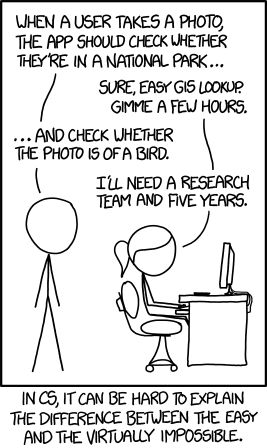
\includegraphics[height=0.8\textheight]{figures/xkcd_tasks} \\
            {\scriptsize%
             From \texttt{xkcd}}
        \end{center}}
    \only<2>{%
        \Large%
        \begin{itemize}
            \setlength{\itemsep}{\medskipamount}
            \item Realise what's possible
            \item Determine existing capacity
            \item Understand the Data Science process
        \end{itemize}}
\end{frame}

\begin{frame}{Don't try to run before you can walk}
    \begin{center}
        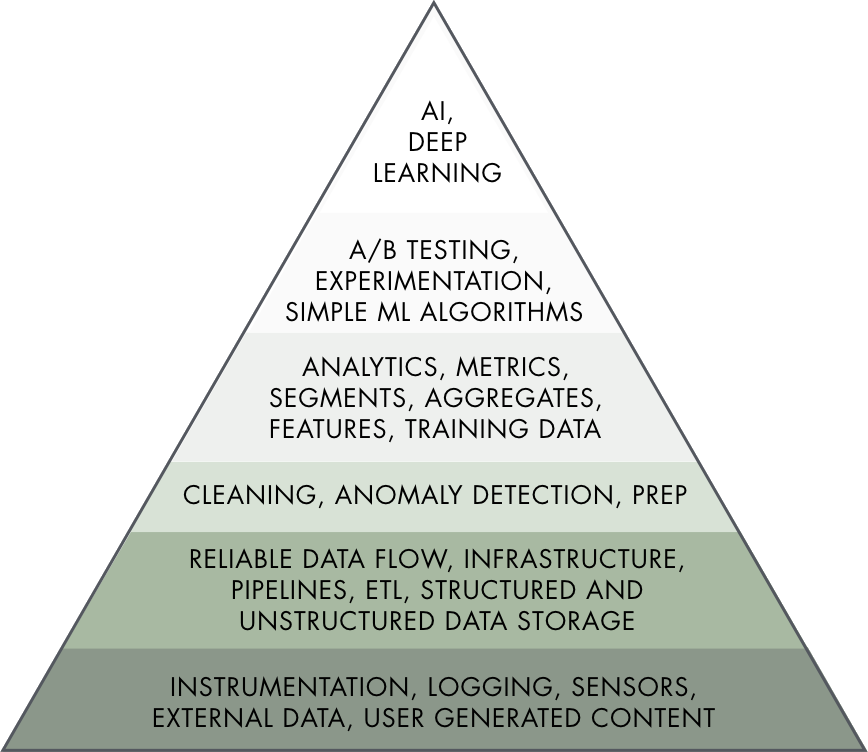
\includegraphics[height=0.8\textheight]{figures/ai_hierarchy} \\
        {\scriptsize%
         From M.\ Rogati}
    \end{center}
\end{frame}

\begin{frame}{Culture}
    \only<1>{%
        \begin{center}
            \Large%
            The ROI of Data Science projects \\
            is very difficult to predict!
        \end{center}
        \vfill
        \begin{itemize}
            \setlength{\itemsep}{\medskipamount}
            \item Power law\hyp{}like distribution of returns
            \item Failure is \emph{always} an option
        \end{itemize}}
    \only<2>{%
        \begin{center}
            \Large%
            Embrace a \\
            \textbf{high\hyp{}risk, high\hyp{}reward innovation culture}
        \end{center}
        \vfill
        \begin{itemize}
            \setlength{\itemsep}{\medskipamount}
            \item Iterate quickly $\to$ fail fast
            \item Operationalise
        \end{itemize}}
\end{frame}

\begin{frame}{Adoption}
    \begin{center}
        {\Large%
         If it's not used in production\ldots}
        \vfill\pause
        {\LARGE\bf%
         It never happened!}
    \end{center}
\end{frame}

\begin{frame}{How to realise the Data Science potential}
    \only<1>{%
        \Large%
        \begin{itemize}
            \setlength{\itemsep}{\medskipamount}
            \item Embed Data Science starting at the top
            \item Build and re\hyp{}build\ldots~fast
            \item Actually use it!
        \end{itemize}}
    \only<2>{%
        \Huge%
        \begin{center}
            How?
        \end{center}}
    \only<3>{%
        \LARGE%
        \begin{center}
            You need \\
            \textbf{good people} and \textbf{good teams}
        \end{center}}
\end{frame}

\begin{frame}{Attracting and retaining good people}
    \Large%
    \begin{itemize}
        \setlength{\itemsep}{\medskipamount}
        \item Have a roadmap
        \item Hire for potential
        \item Let them choose their tools
        \item Give them resources
        \item Nurture their curiosity
    \end{itemize}
\end{frame}

\begin{frame}{Training good people}
    \vspace{2.5em}
    \begin{columns}
        \begin{column}{0.5\textwidth}
            \centering%
            {\Large\bf%
             Data Analyst} \\[\medskipamount]
            \begin{itemize}
                \setlength{\itemsep}{\medskipamount}
                \item Understands the business
                \item Values automation
                \item[$\to$] Teach them the pragmatism of the Software Engineer
            \end{itemize}
        \end{column}
        \begin{column}{0.5\textwidth}
            \centering%
            {\Large\bf%
             Software Engineer} \\[\medskipamount]
            \begin{itemize}
                \setlength{\itemsep}{\medskipamount}
                \item Understands the tech
                \item Knows automation
                \item[$\to$] Train them to recognise what matters to the
                             business
            \end{itemize}
        \end{column}
    \end{columns}
    \pause
    \begin{center}
        \Large%
        Are we up\hyp{}skilling them properly?
    \end{center}
\end{frame}

\begin{frame}{Teamwork}
    \Large%
    A successful Data Science team is\ldots
    \begin{itemize}
        \setlength{\itemsep}{\medskipamount}
        \item Diverse
        \item Flexible
        \item Collaborative
    \end{itemize}
\end{frame}

\begin{frame}{Communication complexity}
    \only<1>{%
        \begin{columns}
            \begin{column}{0.5\textwidth}
                \Large\centering%
                Communication complexity is \\[\medskipamount]
                {\Huge\textbf{quadratic}} \\[\medskipamount]
                in the number of \\
                team members
            \end{column}
            \begin{column}{0.5\textwidth}
                \centering%
                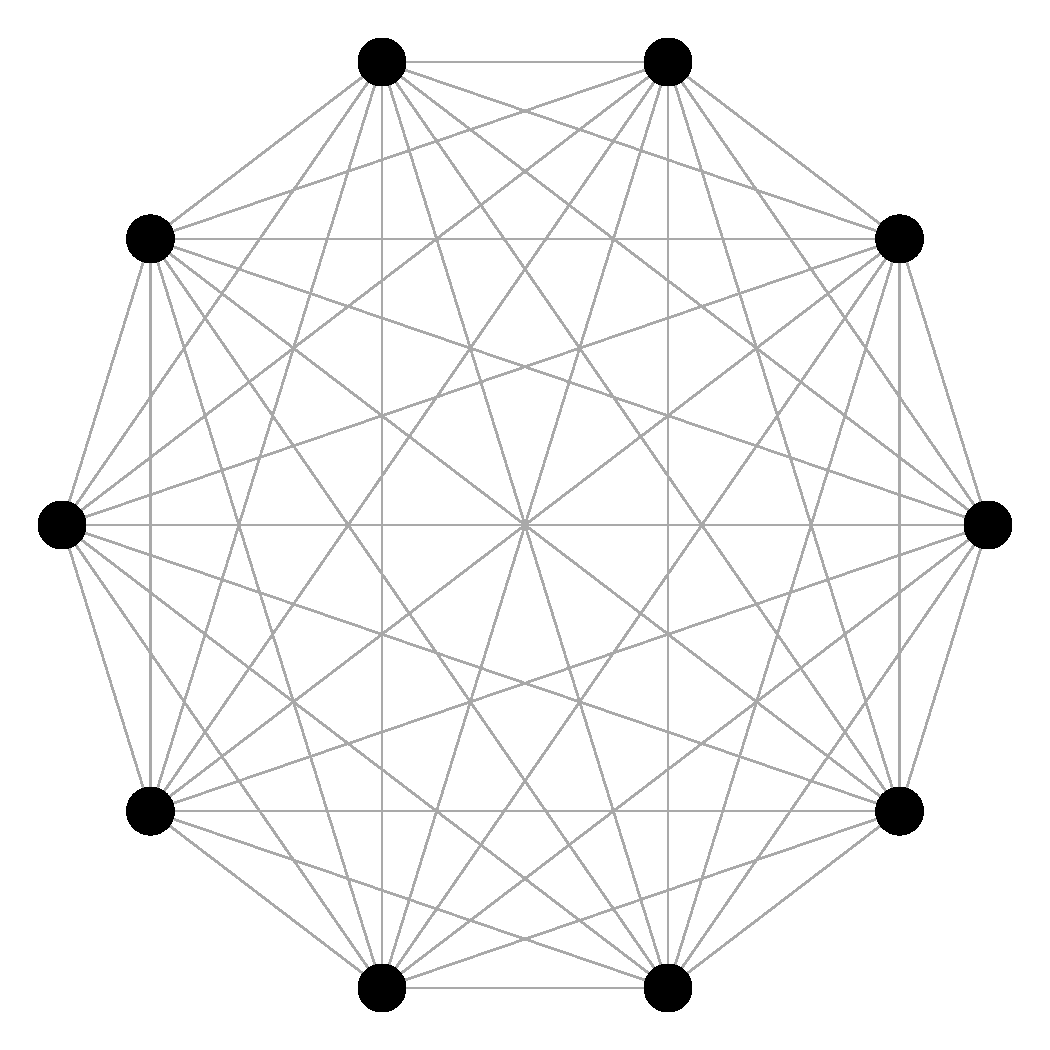
\includegraphics[width=0.8\textwidth]{figures/full_graph}
            \end{column}
        \end{columns}}
    \only<2>{%
        \begin{center}
            \LARGE%
            Make sure there's \\
            \textbf{shared understanding}
        \end{center}
        \vfill
        Particularly of\ldots
        \begin{itemize}
            \setlength{\itemsep}{\medskipamount}
            \item The Data Science workflow
            \item Software Engineering best practices
        \end{itemize}}
\end{frame}

\begin{frame}{Take-aways}
    \Large%
    \begin{itemize}
        \setlength{\itemsep}{\medskipamount}
        \item Embed Data Science and its process
        \item Have a roadmap
        \item Don't look for unicorns
    \end{itemize}
\end{frame}

\end{document}

